\chapter{Распознавание аккордов без использования машинного обучения}
\label{chapt1}

РИСУНОК: общая схема реализованного метода

\section{Частотно-временное представление звукозаписи} \label{sect1_spectrogram}

Западная музыка основывается на равномерно темперированном строе. Поэтому, как
правило, все звуки, издаваемые музыкальными инструментами с определённой высотой
звучания, имеют частоты, соответствующие формуле \ref{eq:note_freq}. В звучании
аккорда, состоящего из нескольих нот, большая часть энергии должна приходиться
на частоты этих нот. Соответственно, разница в звучании двух аккордов должна
выражаться в наличии или отсутствии звуковой энергии на определённых частотах.
Поэтому при построении частотно-временного представления наибольший интерес
представляют частоты, соответствующие звукам западной музыкальной системы. 

\subsection{Определение частоты настройки музыкальных инструментов}
\label{ssect1_f0}

В формуле \ref{eq:note_freq} присутствует параметр $f_0$, задающий частоту
настройки музыкальных инструментов. Как отмечается в \cite{Lerch2012}, с. 89,
некоторые оркестры до сих пор используют частоты настройки 442 Гц и 443 Гц.
Встречающееся гораздо чаще воспроизведение звукозаписи с изменённой скоростью
приводит к аналогичному эффекту, повышая или понижая частоты звучания всех
инструментов композиции. Частоту настройки необходимо определить предварительно,
чтобы избежать ошибок на таких звукозаписях.

Увеличение частоты настройки в $2^{1/12} \approx 1.06$ раз (или примерно на 6\%)
приведёт к повышению звучания инструмента на полутон: вместо звука \emph{си}
будет звучать \emph{до}, вместо \emph{до} -- \emph{до}$\sharp$ и так далее.
Аналогично, повышение скорости воспроизведения в $2^{1/12}$ раз приведёт к
уменьшению периода каждого звука в $2^{-1/12}$ раз, а значит, к повышению
частоты в $2^{1/12}$ раз. Очевидно, в случае такого изменения скорости
воспроизведения невозможно обнаружить сам факт его наличия, не обладая
дополнительной информацией об изначальной тональности композиции. Поэтому обычно
фиксируют диапазон для возможных значений частоты настройки: $[440 \cdot
2^{-1/24}, 440 \cdot 2^{1/24})$, приблизительно соответствующий диапазону от 427
до 452 Гц.

Обзор некоторых алгоритмов определения частоты настройки можно найти в
\cite{Lerch2006} в разделе 4.1. В рамках данной работы используется алгоритм,
похожий на предложенный в \cite{Zhu2005}. Звукозапись делится на короткие
фрагменты между моментами времени $t_m, m = 0, 1, 2, \dots, M'$, на каждом из
которых выполняется constant-$Q$ преобразование с $f_{min} = 440 \cdot
2^{m_0/12}$ для некоторого целого $m_0$, и достаточно высоким разрешением по
частоте: $N_0 = 12 b_0$ компонент на октаву. На каждом фрагменте $C_m = C(t_m)$
определяется номер компоненты $C_m[n]$, $0 \leq n < N'$, которой соответствует
максимальное значение спектра. Затем строится гистограмма значений функции
$C_m[n]$, она состоит из $N'$ столбцов. Значения всех столбцов, номера которых
сравнимы по модулю $b_0$, суммируются. В полученной гистограмме из $b_0$
столбцов номер столбца с наибольшим значением можно интерпретировать как
отклонение $f_0$ от стандартной частоты настройки 440 Гц в диапазоне от -1/2 до
+1/2 полутона с точностью до $1/b_0$ полутона. Если наибольшее значение
приходится на 0-й столбец, то отклонения нет. Используемые здесь значения $M'$ и
$N'$ не обязательно совпадают с соответствующими значениями $M$ и $N$ для
основной спектрограммы.

Допустим, вместо настоящей частоты настройки $f_0$ была ошибочно определена
$f_0' \neq f_0$. Это приведёт к тому, что настоящие частоты звуков будут
отличаться от использованных в преобразовании постоянного качества в $f_0 /
f_0'$ раз.

ЭКСПЕРИМЕНТ: распознавание аккордов с определением частоты настройки и без него.

\subsection{Определение ритма} \label{ssect1_rhyhtm}

Ритм играет важную роль в западной музыке. Так же, как равномерно
темперированный строй упорядочивает звуки по высоте, ритм упорядочивает и
группирует их по времени начала и продолжительности звучания. Поэтому и смена
звучащего аккорда должна происходить в соответствии с ритмом. Наиболее чётко
воспринимаемая человеком пульсация соответствует периодической смене метрических
долей. В дальнейшем будем предполагать, что смена звучащего аккорда всегда
происходит в момент начала какой-то метрической доли. При этом теряется
возможность определения нескольких аккордов в пределах одной метрической доли.
Но расположенные в соответствии с ритмом анализируемые фрагменты позволят
анализировать звук ровно в те моменты, когда музыкальные инструменты звучат
наиболее ярко, и интересующие нас частоты лучше выделены в спектре.

В рамках данной работы для определения ритма в звукозаписях использовались 2
внешние библиотеки: \emph{Beatroot} \cite{Dixon2007} и \emph{Beat tracker}
\cite{Davies2007} из набора \emph{Queen Mary Vamp plugins}. Вторая библиотека
потребовалась для обработки тех композиций, в которых \emph{Beatroot} не
смог определить начала метрических долей.

ЭКСПЕРИМЕНТ: разница в качестве распознавания с использованием одного и другого
биттрекеров.

\subsection{Получение спектра} \label{ssect1_spectrum}

Моменты начала метрических долей $(t_0, t_1, \ldots, t_{M-1})$ и частоты звуков
равномерно темперированного строя образуют сетку на плоскости <<частота-время>>.
Особый интерес представляют значения интенсивности звука, вычисленные в узлах
этой сетки. Информация о моментах начала метрических долей позволяет разделить
звукозапись таким образом, чтобы на каждый из них приходилась середина одного из
фрагментов. Преобразование постоянного качества позволяет на каждом фрагменте
определить интенсивность звука для каждой из указанных частот.

Во многих работах (например, в \cite{Jiang2011}, \cite{Cho2011}) отмечалась
важность сглаживания последовательности столбцов спектрограммы или векторов
признаков. Сглаживание осуществляется путём применения фильтра скользящего
среднего или скользящего медианного фильтра с шириной окна $w$ к каждой строке
спектрограммы. Оно позволяет избавиться от единичных выбросов в спектре, но при
этом несколько размывает спектр, снижая разрешение по времени. Если каждый
столбец спектра соответствует промежутку между двумя метрическими долями, такое
размытие будет слишком сильным.

Чтобы преодолеть этот недостаток, увеличим разрешение спектрограммы по времени в
$T$ раз путём вставки между каждыми моментами $(t_m, t_{m+1})$ равномерно $T-1$
промежуточных значений, где $T$ -- параметр. Тогда появляется возможность
использовать достаточно большой размер окна при сглаживании, не приводящий к
существенному размытию спектра во времени. После сглаживания разрешение
спектрограммы уменьшается в $T$ раз путем удаления добавленных промежуточных
столбцов.

\begin{figure} [h] 
  \center
  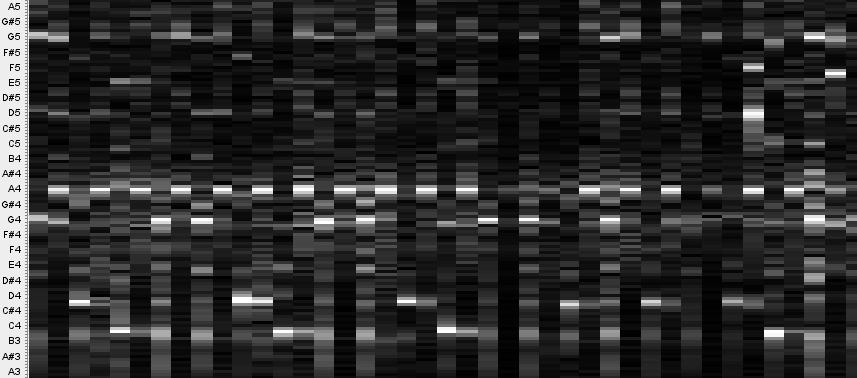
\includegraphics [scale=0.40] {spect_T1c}
  \vspace{20pt}
  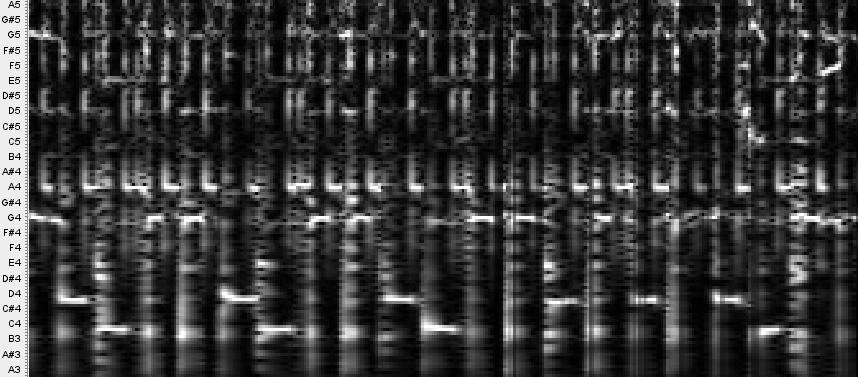
\includegraphics [scale=0.40] {spect_T8c}
  \vspace{10pt}
  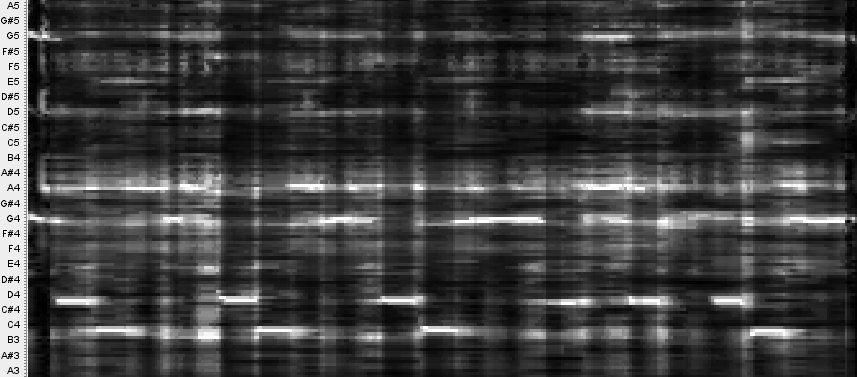
\includegraphics [scale=0.40] {spect_medianc}
  \caption{Фрагменты спектрограммы \emph{The Beatles -- Love Me Do} при $T=1$
  (вверху), $T=8$ (в середине), $T=8$ после сглаживания с $w=19$ (внизу).}
  \label{img:spectT}  
\end{figure}

Равномерно темперированный строй предполагает расположение $N_0=12$ ступеней
звукоряда в пределах октавы, поэтому удобно выбирать $N_0$ кратным $12$. Большие
значения $N_0$ дают возможность в некоторой мере скомпенсировать ошибки при
определении частоты настройки музыкальных инструментов $f_0$, позволяя учесть
близкие к $f_k = 2^{k/12} f_0$ частоты. В \cite{Bello2005}, \cite{Lee2006},
\cite{Mauch2008}, \cite{Oudre2009}, \cite{Cho2010}, \cite{Cho2011}
использовалось значение $N_0=36$. Как показано ниже, $N_0=60$ позволяет добиться
лучшего результата.

\begin{figure}[h]
  \begin{minipage}[h]{0.49\linewidth}
    \center{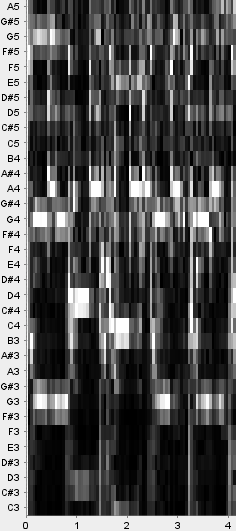
\includegraphics[width=0.5\linewidth]{spect_b12c} \\ а)}
  \end{minipage}
  \hfill
  \begin{minipage}[h]{0.49\linewidth}
    \center{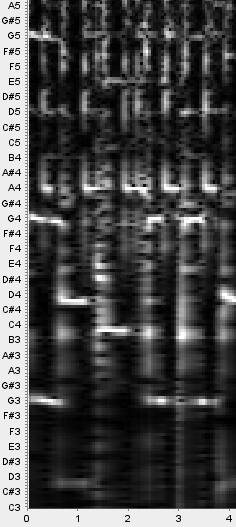
\includegraphics[width=0.5\linewidth]{spect_b60c} \\ б)}
  \end{minipage}
  \caption{Фрагменты спектрограммы \emph{The Beatles -- Love Me Do} при: а)
  $N_0=12$; б) $N_0=60$.}
  \label{img:spectb}  
\end{figure}

Важно также правильно выбрать частоту наименьшей из компонент преобразования
$f_{min}$ и общее количество компонент $N$. Они определяют используемый для
анализа частотный диапазон. Обычно используются частоты в пределах 50-2000 Гц.
В \cite{Weller2009} используемый диапазон ограничен сверху 1000 Гц, а в
\cite{Cho2011} -- 4186 Гц. Для определения более частот ниже 50 Гц требуется
слишком длинный фрагмент звука, а частоты выше 2000 Гц обычно содержат только
гармоники более низких нот, затрудняющие определение аккорда.

ЭКСПЕРИМЕНТ: сравнение качества распознавания для $N_0$=12,36,60, и
охвата в 4,5,6 октав.
ЭКСПЕРИМЕНТ: сравнение с БПФ при тех же условиях (с определением ритма и частоты
настройки).

%\newpage
%============================================================================================================================

\section{Выделение мелодических компонент спектра и векторы признаков}
\label{sect1_feat}

На этом этапе к спектрограмме применяется серия преобразований. Они нацелены на
акцентирование компонент, которые несут важную для идентификации аккорда
информацию, и на подавление остальных компонент. Наиболее важным является
подавление шума и инструментов с неопределенной высотой звучания, поскольку их
спектр не зависит от звучащего аккорда и сопоставим по уровню со спектром
инструментов, задающих аккорд.

РИСУНОК: спектр с четко выраженными ударными и гитарой и вокалом

Как видно из рисунка, барабан оставляет на спектрограмме яркие вертикальные
полосы. В то же время, гитаре соответствуют горизонтальные полосы. Это свойство
используют алгоритмы разделения звука на гармонические и перкуссионные
компоненты, такие как \cite{Ono2008} и \cite{Fitzgerald2010}. В данном случае
полное разделение является излишним, необходимо только подавить перкуссионные
компоненты.

Маух в \cite{Mauch2010} предложил вычитать из спектрограммы так называемый
фоновый спектр. При этом каждое значение спектрограммы $C_m[n]$ заменять на
$\frac{C_m[n] - \mu_m[n]}{\sigma_m^q[n]}$, где $\mu_m[n]$ представляет собой
среднее значение, а $\sigma_m^q[n]$ -- среднеквадратическое отклонение в
пределах отрезка от $C_m[n-k]$ до $C_m[n+k]$, охватывающего одну октаву, $q \in
\{0, 1\}$. Если полученное значение является отрицательным, вместо него
подставляется 0.

Автором в \cite{Glazyrin2012} было предложено использовать аналог фильтра
Превитт, используемого в обработке изображений для выделения границ. Будем
для каждого фрагмента спектрограммы размера $9 \times 3$ с центром в точке
$C_m[n]]$ вычислять его свёртку с матрицей
$$P = \begin{pmatrix}
-1 & -1 & -1\\
-1 & -1 & -1\\
-1 & -1 & -1\\
2 & 2 & 2\\
2 & 2 & 2\\
2 & 2 & 2\\
-1 & -1 & -1\\
-1 & -1 & -1\\
-1 & -1 & -1\\
\end{pmatrix}$$
Если полученное значение больше 0, то заменим $C_m[n]$ на него, иначе -- на 0.

\begin{figure}[h]
  \begin{minipage}[h]{0.49\linewidth}
    \center{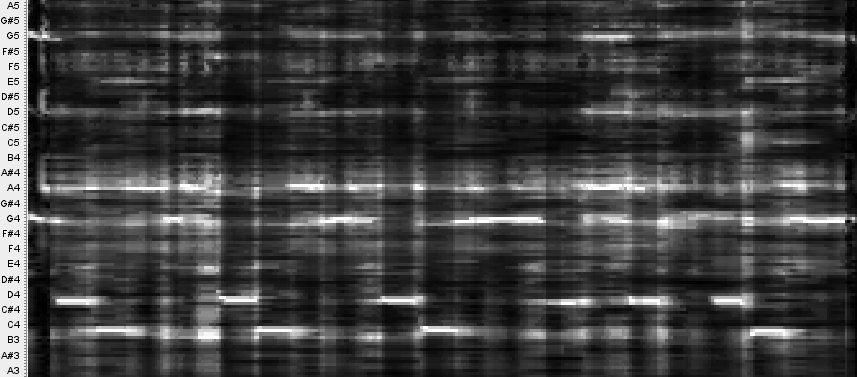
\includegraphics[width=0.9\linewidth]{spect_medianc} \\ а)}
  \end{minipage}
  \hfill
  \begin{minipage}[h]{0.49\linewidth}
    \center{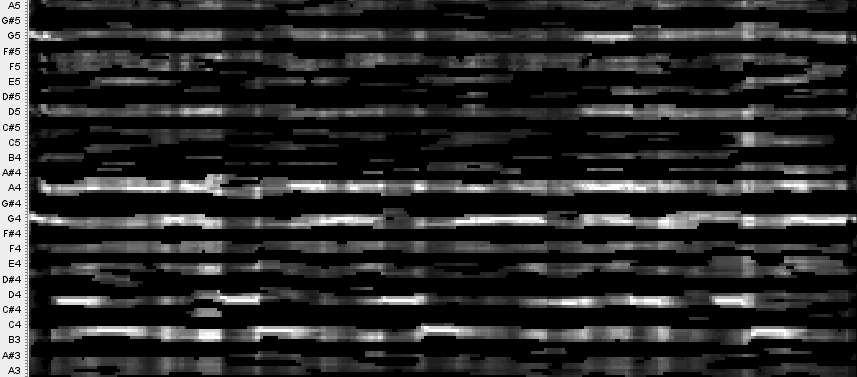
\includegraphics[width=0.9\linewidth]{spect_prewittc} \\ б)}
  \end{minipage}
  \caption{Фрагменты спектрограммы \emph{The Beatles -- Love Me Do}: а)
  до применения фильта Превитт; б) после применения фильта Превитт.}
  \label{img:spectb}  
\end{figure}

Еще один подход к подавлению перкуссионных компонент лёг в основу алгоритма
вычисления признаков CRP \cite{Mueller2009}. Будем рассматривать $C_m[n]$ как
сигнал (количество энергии, приходящейся на данную частоту, в зависимости от
частоты). Применим к этой функции дискретное косинусное преобразование.
$$ DC_m[k] = \sum\limits_{j=0}^{N-1} C_m[j] \cos\left[ \frac{\pi}{N} \left(
j+\frac{1}{2} \right) k \right], \quad k=0, \ldots, N-1 $$
В полученной последовательности значений занулим первые $\xi$ значений, после
чего произведём обратное дискретное косинусное преобразование. Зануляемые первые
коэффициенты соответствуют низкочастотным компонентам сигнала $C_m[n]$, которые,
в свою очередь, соответствуют достаточно длинным последовательностям существенно
отличных от нуля значений.

Как показывает практика, важным шагом является применение к спектрограмме
логарифмического преобразования: каждая компонента $C_m[n]$ заменяется на
$\log_{10}(1000 C_m[n] + 1)$. После него соотношения между компонентами
спектрограммы лучше соответствуют человеческому восприятию интенсивности звука.

РИСУНОК: столбец спектрограммы до ДКП и после ДКП-зануление-ОДКП.
РИСУНОК: спектрограмма до логарифмического преобразования и после него.
ЭКСПЕРИМЕНТ: сравнение качества распознавания с применением разных методов
очистки.

\section{Применение самоподобия} \label{sect1_selfsim}

Важным свойством музыкальных звукозаписей является наличие повторений. Музыка
нравится человеку в том числе из-за повторений одного и того же мотива в разных
вариациях, с некоторыми изменениями. Во многих композициях имеется достаточно
продолжительный повторяющийся припев. В рамках куплета может повторяться одна и
та же музыкальная фраза длительностью в несколько тактов. Можно попытаться
использовать повторения для улучшения спектрограммы.

В работах \cite{Mauch2010} и \cite{Cho2011} повторяющиеся фрагменты композиции
использовались для улучшения качества распознавания аккордов. В обеих методах
строились матрицы самоподобия для 12-мерных хроматических вектороов признаков с
использованием в качестве меры подобия коэффициента корреляции Пирсона (в
\cite{Mauch2010}) и евклидового расстояния (в \cite{Cho2011}). В полученной
матрице находятся линии, параллельные главной диагонали, которые соответствуют
похожим друг на друга фрагментам. Эти фрагменты затем используются для
дополнительного сглаживания спектрограммы.

Однако матрицу самоподобия можно строить и для столбцов спектрограммы
$\{C_i\}_{i=0}^{M-1}$, каждый из которых содержит больше информации по сравнению
с соответствующим вектором признаков. Обозначим эту матрицу за $\{s_{ij}\}$, где
$s_{ij}$ -- евклидово расстояние между столбцами $C_i$ и $C_j$. Эта матрица
имеет нули на главной диагонали. Нормализуем её таким образом, чтобы $0 \leq
s_{ij} \leq 1$ для всех $i, j$. Затем в каждой строке сохраняются $\zeta \cdot
M$ наименьших значений ($0 \leq \zeta \leq 1$), а все остальные заменяются на 1.

При помощи полученной матрицы можно скорректировать все столбцы $C_m$:
$$
\widehat{C}_m = \frac{\sum\limits_{j=0}^{M-1} (1 - s_{mj})
C_j}{\sum\limits_{j=0}^{M-1} (1 - s_{mj})} $$

РИСУНОК: матрица самоподобия
ЭКСПЕРИМЕНТ: сравнение качества распознавания со сглаживанием и без него

%\newpage
%============================================================================================================================

\section{Классификация и исправление ошибок} \label{sect1_class}

\subsection{Классификация хроматических векторов} \label{ssect1_chroma}

Будем рассматривать в качестве множества возможных названий аккордов $Y$ набор
из названий 24 мажорных и минорных аккордов и символа <<N>>, означающего
отсутствие аккорда. За основу возьмём метод ближайшего соседа с шаблонами,
учитывающими основной тон и 3 первых обертона по формуле
(\ref{eq:templates_harmonics}). Эти шаблоны задаются для 12-мерных хроматических
векторов. Столбцы спектрограммы охватывают несколько октав, поэтому для каждого
из них потребовалось бы несколько шаблонов, чтобы учесть все возможные
сочетания октав, в которых могут располагаться ноты аккорда.

ЭКСПЕРИМЕНТ: зависимость качества распознавания от количества гармоник в
шаблонах.

Для получения 12-мерных хроматических векторов сначала ко всем значениям
$\widehat{C}_m[n], ~ 0 \leq n < N_0$, прибавляются значения
$\widehat{C}_m[n+N_0], ~ \widehat{C}_m[n+2N_0], ~ \widehat{C}_m[n+3N_0], ~
\ldots$ для каждого $0 \leq m \leq M-1$, давая в результате последовательность
$N_0$-мерных векторов $\{B_m\}_{m=0}^{M-1}$. Далее в случае $N_0=12 b_0, ~ b_0
\geq 3$ каждый вектор $B_m$ преобразуется в 12-мерный вектор $D_m$:
$$ D_m[n] = B_m[b_0 n - 1] + B_m[b_0 n] + B_m[b_0 n + 1], \quad m=0,\dots,M-1,
\quad n=0,\dots,11 $$ 
Для вычисления $D_m[0]$ в качестве $B_m[-1]$ используются $B_m[59]$.

Для каждого из последовательности векторов $\{D_m\}_{m=0}^{M-1}$ определяется
ближайший из шаблонов, и соответствующий ему аккорд считается аккордом, звучащим
на данном фрагменте.

\subsection{Исправление ошибок классификации} \label{ssect1_errcorr}

В результате экспериментов было обнаружено, что некоторые последовательности
аккордов являются маловероятными в реальной композиции, и скорее всего является
ошибочными. Для двух классов таких последовательностей предлагается метод их
исправления.

\subsubsection{A:maj - A:min}

К первому классу относятся последовательности, в которых аккорды имеют общую
основную ноту, но различные типы, например: A:maj-A:min-A:maj-A:min. Появление
таких последовательностей возможно, поскольку соответствующие векторы признаков
достаточно близки друг к другу. Для каждой такой последовательности находится
вектор признаков, являющийся средним арифметическим составляющих её векторов.
Аккорд, соответствующий полученному вектору признаков, приписывается всей
последовательности.

\subsubsection{A-B-C}

Ко второму классу относятся последовательности из 3 разных идущих подряд
аккордов: A-B-C (при этом возможно A=C). В этом случае более вероятно, что на
самом деле имел место один из следующих 4 вариантов: A-A-C, A-C-C, A-B-B,
B-B-C. Из них выбирается тот, для которого сумма расстояний от векторов
признаков до соответствующих шаблонных векторов минимальна. Очевидно, что такая
коррекция будет ошибочной в тех случаях, когда аккорд действительно звучит
только в течение одной метрической доли.

ЭКСПЕРИМЕНТ: качество распознавания до и после применения эвристик
ПРИМЕРЫ композиций, где это работает и где не работает

\section{Выводы}

TODO

%\newpage
%============================================================================================================================

\clearpage